%
% Annual Cognitive Science Conference
% Sample LaTeX Paper -- Proceedings Format
%

% Original : Ashwin Ram (ashwin@cc.gatech.edu)       04/01/1994
% Modified : Johanna Moore (jmoore@cs.pitt.edu)      03/17/1995
% Modified : David Noelle (noelle@ucsd.edu)          03/15/1996
% Modified : Pat Langley (langley@cs.stanford.edu)   01/26/1997
% Latex2e corrections by Ramin Charles Nakisa        01/28/1997
% Modified : Tina Eliassi-Rad (eliassi@cs.wisc.edu)  01/31/1998
% Modified : Trisha Yannuzzi (trisha@ircs.upenn.edu) 12/28/1999 (in process)
% Modified : Mary Ellen Foster (M.E.Foster@ed.ac.uk) 12/11/2000
% Modified : Ken Forbus                              01/23/2004
% Modified : Eli M. Silk (esilk@pitt.edu)            05/24/2005
% Modified : Niels Taatgen (taatgen@cmu.edu)         10/24/2006
% Modified : David Noelle (dnoelle@ucmerced.edu)     11/19/2014

%% Change "letterpaper" in the following line to "a4paper" if you must.

\documentclass[11pt,letterpaper]{article}

\usepackage{booktabs}
\usepackage{caption}
\usepackage{subcaption}
\usepackage{setspace}
\usepackage{hyperref}
\usepackage{multirow}
\usepackage{minted}
% \usepackage{lineno}
% \linenumbers
% \usepackage{cogsci}
\usepackage{pslatex}
\usepackage{apacite}
\usepackage{amsmath}
% \usepackage{authblk}
\usepackage{graphicx}
\usepackage[margin=1.25in]{geometry}

% \doublespace


\title{Cable news, politics, and metaphorical violence}

\author{Matthew A. Turner}

\begin{document}

\maketitle


\begin{abstract}
People rarely think twice about metaphorical violence when talking about 
political debate, strategy, and elections. But we should think twice because
such talk has real-world consequences. Before we can think twice about how we
talk about politics we need to know exactly what is said about politics. What language
we use depends on what is going on around us, so we must also know when our
language is apt to change and what might be driving that change. In a corpus analysis
of metaphorical violence on cable news, I show that metaphorical violence increases
around the the presidential debates 
preceding the United States presidential election of 2016. In support of this
analysis, I also present two novel, reusable, and open-source software packages. 
The first provides free, programmatic access to cable news archives hosted
by the Internet Archive. The second is Metacorps: a data model, web application,
and analytical pipeline for efficient, collaborative metaphor coding across corpora. 
These two software packages feed a statistical analysis that pinpoints when metaphorical
violence usage increases, and quantifies the level of increase, under the
influence of the presidential debates. This study increases our understanding of the
dynamics of metaphorical violence in the realm of politics. Such understanding
is important for the design of behavioral studies, 
which in turn will lead to a healthier democracy through more inclusive and 
effective political communication.

\end{abstract}

\newpage

\section{Introduction}
Language, thought, and behavior are inextricably linked. In certain extreme
cases, like an army general giving orders, the links between the three clear. 
In other cases, like politics, the chain of events is less clear. Did some
political behavior cause thought, which produced a certain utterance? Was a
conceptual cascade triggered by something that was said? Did someone not vote
because of what they heard on television? Language has the ability to reinforce
or alter the relationships between concepts in our mind. Similarly, the relationship
between concepts in our mind drive how we talk about things. Not only do
relationships between concepts drive utterances, but the relationship between
speaker and audience also drives what is said. In many cases, pragmatic choice,
what is said and how, is made at an unconscious level. However, that does not mean
that the way a particular issue is commonly framed is optimal. In fact, to 
communicate as effectively as possible with the best outcomes, we need to check
whether what we say fits with our goals and values. We need to evaluate the
conceptual structures that have become established in our own mental space and
the mental space of society as a whole. The first step towards evaluating
our concepts and language is understanding what we say and why we say it. 
This paper examines a specific and ubiquitious conceptual structure that may
pose challenges for effective democratic decision-making: the general conceptual metaphor
\textsc{politics is a physical conflict}. I show that this results in metaphorical
violence usage increasing on cable news shows around the days of the 2016 
presidential debates. Furthermore, I pinpoint the exact date increased metaphorical
violence usage on cable news begins and the exact date it ends. This provides
the much needed starting point for us to ask whether or not such language
use is healthy for democracy.

While metaphorical violence in politics may be normal, we should not underestimate its
importance or assume it has no real-world consequences. 
Its effects are more than increased rhetorical power. 
When more aggresive people read political messages containing mild metaphorical violence, 
their support for political violence increases. Less aggressive people tend to
lose faith in government efficacy when they are exposed to metaphorical violence
in political messaging \cite{Kalmoe2014}. 
In an extreme but important example of this, Representative
Gabrielle Giffords' Arizona congressional district was overlaid with a gun sight. 
She was among 20 house democrats who were singled out for voting for the 
Affordable Care Act. The map was produced by Sarah Palin's political action 
committe SarahPAC. Palin herself announced the campaign to retake the house 
seats, tweeting ``Commonsense Conservatives \& lovers of America: `Don't Retreat,
Instead - RELOAD!' Pls see my Facebook page.'' This tweet was published March
23, 2010. In January, 2011, following the 2010 congressional elections, 
Representative
Giffords was shot at a ``Congress on your Corner'' event at a Safeway in 
Tuscon, Arizona. She miraculously survived a headshot wound, but six others
were killed including a Federal judge and a nine-year-old girl. Fifteen were
wounded. As Giffords herself said in an interview on MSNBC nine months before
the attack ``we've gotta realize that there are consequences to that action...we have to work out 
our problems by negotiating and working together.''

Elections are an improvement over violent struggles for power. However, this
has not eliminated all political violence, and it certainly has not elminated
metaphorical violence from discourse about debates and elections. 
Metaphor is an essential human cognitive capability. We understand abstract
concepts, like a debate, in terms of embodied experience, like a fight. Possibly
because of the fact that elections replace violent transfers of power, 
English-speaking Americans are inundated with metaphorical violence describing
political messaging and debate strategy. Language is often underspecified, 
meaning many details are left out. Metaphorical violence leaves individual 
listeners to fill in details
themselves. For example, on Fox News' \textit{The Kelly File}, Megyn Kelly
gave Donald Trump advice on how to ``fight'' against Hillary Clinton in the
second presidential debate: ``Punch back. Don't defend everything she lobs your
way, don't be on defense. But punch back. Punch at her, and punch relentlessly,
actually, as the night goes on.'' We might hear something like this at home,
at a restaurant, in a waiting room, or in the airport. But taken out of context,
we can't know that Megyn Kelly is talking about a debate. She might well be
talking about Ronda Rousey's strategy in an upcoming Ultimate Fighting Championship
cage match.

What is metaphor exactly, and how does it work in general? The ability to 
think and communicate with metaphor is a basic human cognitive ability.
\textit{Conceptual metaphor} is used to relate two or more 
concepts.  Typically one of the concepts is more abstract and the other is
more concrete, or \textit{embodied}, meaning it's something we've physically
experienced. We understand the abstract concept in terms of the more embodied
concept. For example, a recurring conceptual metaphor in political discourse
is \textsc{a debate is a fight}. Conceptual metaphors by convention are written
in small caps. The first concept is called the target domain and the second 
concept is called the source domain. Elements of the source domain, the embodied
domain, are mapped on to the target domain. In \textsc{a debate is a fight}, 
the rather abstract concept of a debate is understood in terms of particular
elements of a fight, such as heightened emotions, the importance of
strategy, and the necessity of endurance. Importantly, metaphor also hides 
certain, sometimes fundamental, elements of the target domain. In understanding
a presidential debate as a fight, we ignore the ultimate purpose of such debates:
to identify which candidate's plans would most benefit us as individuals and
the nation as a whole. Framing debates as a fight assumes that there must be
a winner and a loser, with no other redeeming features of the outcome. While
a fight may be decided by the quality of a fighter's strategy, the strategy is
hidden from most observers. On the other hand, in a debate we should pay careful
attention to the reasoning and rationale behind the contestants' statements.
We should base our voting behavior not on who won or lost in the sense of a
fight, but instead who presented better policy with more convincing arguments.
Such conceptual relationships are expressed as linguistic instances of metaphor,
which are the behavioral data collected in this study. 

There are real consequences to the exaggeration of certain elements of debate and
hiding others.  As such, this work expands our understanding of how
metaphorical violence is used on cable news. Cable news is watched in millions
of households every night when it's broadcasted, watched by millions more online, 
and showed at restaurants, airports, and waiting rooms across the country.
From cable news alone, we are bombarded with metaphorical violence. Cable news
also provides us with convenient, if inexact, representations of the 
political left, center, and right, by different channels. MSNBC is the 
left-leaning channel, CNN represents the center, and Fox News represents
right-wing ideologies \cite{Bode2014}. Cable news as a source for corpora is 
especially enlightening
because it must satisfy a number of communicative requirements. First, it must present some
trustworthy semblance of the true nature of current events. Secondly, it must
communicate current effects effectively to its audience, meaning cable news
channels must adopt language that is easily understood by its viewers. Third,
cable news channels must reinforce conceptual relationships deemed profitable---this
may include perpetuating political biases or avoiding negative coverage of
sponsors. People form emotional attachments to the anchors, even considering them
family members. \citeA{Hochschild2016} interviewed a conservative person from
Louisiana who described various Fox News anchors: 
"'Bill O'Reilly is like a steady, reliable dad. Sean Hannity is like a difficult uncle who rises to anger too quickly. Megyn Kelly is like a smart sister.'" We need to think critically
about what impact all this has on democratic participation.

Very little systematic work has been done examining the dynamics of metaphor use over time,  
especially on a daily timescale, as presented here, and especially regarding 
metaphorical violence about politics on cable news. 
Cable news data itself is not straight-forward to 
acquire. The Vanderbuilt cable news database is one resource, but it is 
not publically available---one's institution must pay for access. 
The software tools I present here, combined
with the immense database hosted by the Internet Archive, 
provide a novel, open, and programmatic way to access large amounts of cable news data. 

Metaphor has been extensively studied as it relates to politics. 
However, metaphor is typically studied without any explicit
dependence on what is going on inside or out of the discursive environment
that produced the metaphor.  
The work presented here expands our knowledge of
how metaphor use changes over time in response to political events \cite{Gibbs1997}. 
We know, for example, that metaphors for war hide the subleties and realities of armed
conflict \cite{Lakoff1991}. \citeA{Lakoff2004, Lakoff2008}, and \citeA{Lakoff2012} 
identify existing conceptual metaphors and their linguistic instantiations. They
argue that the two major political divisions
of the United States, liberal and conservative, each have their own 
specialization of
the general conceptual metaphor \textsc{the nation is a family}. For liberals
the family is a ``nurturing parent family'' where the parents' genders are
unimportant and children are loved first and disciplined second; discipline is
never violent. On the other hand, conservatives are supposed to conceptualize
the nation as a ``strict-father family.'' In this family, parents hold to 
rigid gender roles, children are punished with violence, homosexuality and
abortion are both threats to future generations of strict-father families.
This series of work is aimed at liberals and progressives with the goal of 
making their language more convincing to the general public. So, implicitly, 
language is assumed to be changable. But here we make this assumption explicit
and investigate the direct relationship between metaphorical violence and 
the political event of United States presidential debates.

% We know some facts about why metaphor is used in politics
% Another framework to mention is that of 
% \citeA{Charteris-Black2009}, which claims the ultimate goal of metaphor in
% politics is ``forming legitimacy.'' This is done through four main types of 
% metaphors: ``metaphors that establish ethical integrity,'' ``metaphors that
% communicate political arguments,'' ``metaphors that heighten emotional impact,''
% and ``metaphors that communicate ideology and political myth.'' These frameworks
% are useful, but do not bring us closer to understanding the dynamics of
% metaphor use over time. When certain metaphors are used, and why are particular
% metaphors are used? The aim of this work is to 
% find explicit evidence of the connection between the presidential debates of 
% the 2016 United States elections and the usage of metaphorical violence on 
% cable news. In the process, I built software that enables more efficient
% large-scale analysis and annotation of metaphor in a corpus. I also introduce 
% a statistical method for finding when and how general language use changes, 
% which I apply to this particular case of finding when and how much 
% metaphorical violence usage increases.

Using cable news transcripts from a three-month period, September to November, 2016, 
I show that metaphorical violence usage
increased on cable news around the time of the presidential debates. By 
marking each date as either ``normal'' or ``elevated,'' as in normal levels
of metaphorical violence usage or elevated levels of metaphorical violence
usage, and fitting a simple linear model, I found that metaphorical violence
usage did in fact increase from about 1 instance per episode per day to 
2.7 instances per episode per day. This was for the top two shows on each network, MSNBC,
CNN, and Fox News. Furthermore, by varying which days were coded ``normal''
and ``elevated,'' I pinpointed the exact date the increase in usage started and
ended: the elevated usage began September 25 and ended October 26. For reference,
the first debate was September 26 and the final of three debates was October
19. So, increased usage of metaphorical violence nearly exactly coincides with
the first debate, and continues after the last debate for about a week. However
the exact end date is less exactly determinable, possibly due to the election
on November 8.


\section{Methods}
\label{sec:Methods}

First in this section the corpus and the method for building the corpus are introduced. Then
a new web-based application for collaborative metaphor annotation and coding 
is introduced.  This tool allows for efficient export, including a data 
analysis pipeline API for custom Python applications.  
The methods for data export and analysis are demonstrated. Finally, the
statistical methods used for finding the phase transitions in figurative 
violence use are discussed.

\subsection{Corpus}
\label{subsec:Corpus}

The corpus is a set of 607 transcripts from cable news shows aired from
September 1, 2016 to November 30, 2016 (inclusive). The transcripts were from
six shows from three networks, Fox News, MSNBC, and CNN. The shows were the
two most watched shows from each network for the month of
October, 2016 \cite{Katz2016}. The shows and their networks are listed in 
Table \ref{tab:shows}. 

\vspace{.2in}

\begin{table}[!htb]
  \centering
    \begin{tabular}{|c|c|}
      \hline
        Network & Programs \\
      \hline
      \multirow{2}{*}{Fox News} 
        & The O'Reilly Factor \\
        & The Kelly File \\
      \hline
      \multirow{2}{*}{MSNBC}
        & The Rachel Maddow Show \\
        & The Last Word with Lawrence O'Donnell \\
      \hline
      \multirow{2}{*}{CNN}
        & Anderson Cooper 360 \\
        & Erin Burnett OutFront \\
      \hline
    \end{tabular}
  \caption{List of shows used in corpus and their networks.}
  \label{tab:shows}
\end{table}

While the transcripts may be available on each network's website 
for each of the days in the study range, we don't depend on this.
Instead, we use the Internet Archive's (\url{http://archive.org}) 
TV News Archive, or TVNA for short (\url{http://archive.org/tv/details}).
There are several reasons that the TVNA is prefereable to scraping network
websites for transcripts.
First, there is no guarantee that everything said on the show
will be in the transcript. The transcripts used here are built from the
closed captioning recorded and stored in the TVNA. 
Second, the Internet Archive provides a stable, though hidden, API for 
programmatic access to the data stored there. Therefore, the software built
for corpus building does not have to scrape multiple websites, it only needs to
scrape one. Included with calls to the TVNA is a wealth of metadata on each
show including the original air date, run time, links back to the TVNA, and
clip download links. These are all used to build rich software for corpus
building and annotation as demonstrated below.


\subsubsection{iatv: open source tool for TVNA scraping}
\label{subsec:iatv}

To access the data on the TVNA, I developed a new, open-source 
software tool in the Python programming language called \textit{iatv}
\cite{Turner2016}. More details can be found on the GitHub repository page
at \url{http://github.com/mtpain/iatv}. But as a brief example, here is
how one would download all transcripts and the associated metadata from
all shows aired on Fox News in September, 2016

\begin{minted}[fontsize=\small]{python}
from iatv import search_items, download_all_transcripts

# search string cannot be empty so use 'I'; set rows=1000 to get all shows 
items = search_items('I', channel='FOXNEWSW', time='201609', rows=1000)

# filter out commercials
shows = [item for item in items if 'commercial' not in item]

# base_directory will be created or overwritten by default
download_all_transcripts(shows, base_directory='FOXNEWSW-Sep2016')
\end{minted}

Here is an example of the directory structure of \texttt{base\_directory}, which
has been set to \texttt{FOXNEWSW-Sep2016}.

{\small
\begin{verbatim} 
FOXNEWSW-Sep2016
|
+-FOXNEWSW_20160901_000000_The_OReilly_Factor
|   |
|   +-FOXNEWSW_20160901_000000_The_OReilly_Factor.cc5.srt
|   +-metadata.json
|   +-transcript.txt
|
+-FOXNEWSW_20160901_010000_The_Kelly_File
|   |
|   +-FOXNEWSW_20160901_010000_The_Kelly_File.cc5.srt
...
\end{verbatim}
}

\noindent
The \texttt{base\_directory} is populated with subdirectories named by the Internet
Archive's ID for the program. Within each of those subdirectories, there is
the raw \texttt{.srt} file, containing the SubRip-formatted captions 
\cite{Matroska2016}, a metadata file containing all metadata obtained from the
TVNA, and a text file of the transcript converted from the \texttt{.srt} using
\href{https://github.com/pbs/pycaption}{PBS's \texttt{pycaption} library} for Python
\cite{PBS2016}. This concludes the first step in the data acquisition and
processing pipeline, continued in the following sections.


\subsection{Metacorps: Web app and API for corpus annotation and analysis}
\label{sub:corpus-annotation}

Here we introduce the web application and underlying data model that allows us
to collaboratively code instances of metaphor using the \texttt{FOXNEWSW-Sep2016} as
an example. This process is implemented using the 
\href{http://github.com/mtpain/metacorps}{\texttt{metacorps} package} I developed
as part of this project \cite{Turner2017}. 
The package includes both the web application
front-end for collaborative metaphor coding and an API for building the 
specific datasets to be analyzed, including searching for relevant violent
words and phrases. 

In the first step of this process, we insert the data and metadata
acquired from the TVNA into a MongoDB database. No further pre-processing is done 
at this point.
Each subdirectory in the \texttt{FOXNEWSW-Sep2016} is considered an \texttt{IatvDocument},
which is represented as a Python class. All MongoDB collections are represented
as Python classes, using the \texttt{mongoengine} document-object mapping software
\cite{Mongoengine2017}. Then specific documents are selected for analysis, 
building a separate corpus under the collection \texttt{IatvCorpus}. 
An \texttt{IatvCorpus} is then used to build another collection type, a
\texttt{Project}. In building the project, a list of 
violent words or phrases that may be used figuratively must also be given.
Each of these words defines a \texttt{Facet}, and each \texttt{Facet} is comprised
of a list of \texttt{Instance} types. Instances are potential figurative uses
of violence. These instances are what are reviewed by annotaters.
In the web interface, the reviewers can read the paragraph in which the
instance occurred, mark whether the instance was indeed figurative, whether to
include it in the analysis (it may be figurative but not related to politics),
the underlying conceptual metaphor, the perpetrator and victim of violence,
the tense, and whether or not the construction is active or passive. A 
screenshot of the facet navigation page and the \textit{attack} instance
navigation and viewing page are shown in Figure \ref{fig:metacorps-screenshots}.

\begin{figure*}[t!]
    \centering
    \begin{subfigure}[b]{0.45\textwidth}
        \frame{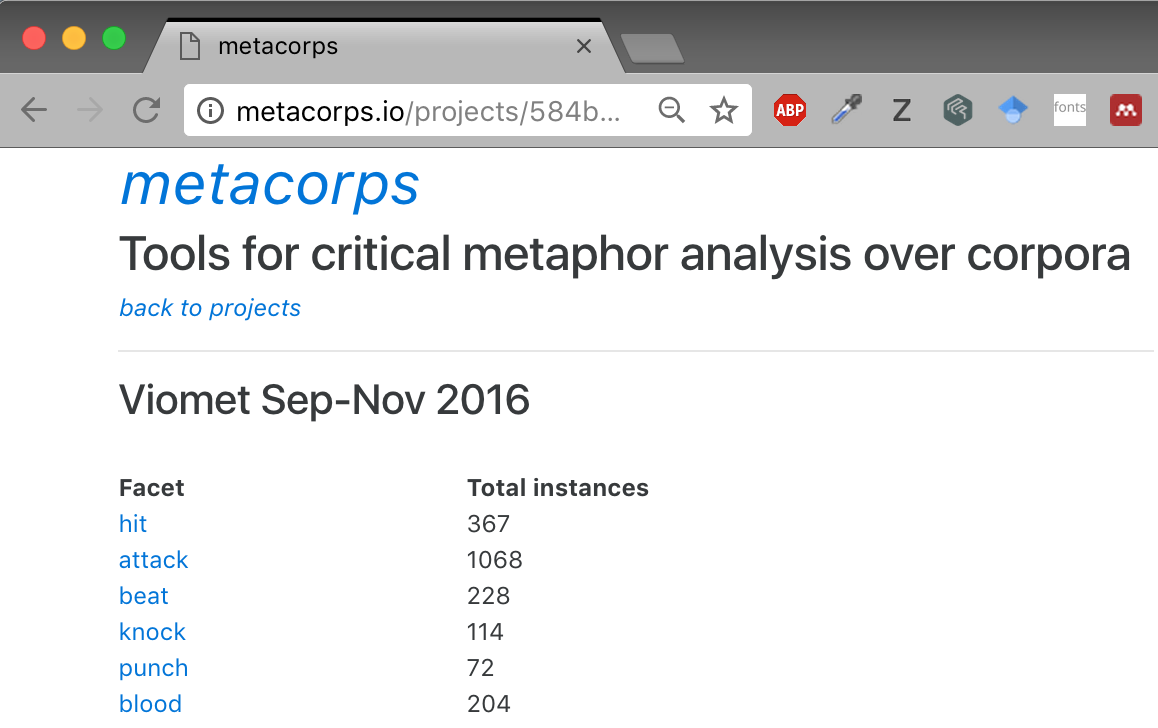
\includegraphics[width=\textwidth]{figures/facet-view.png}}
        \caption{Facet navigation}
    \end{subfigure}
    ~
    \begin{subfigure}[b]{0.45\textwidth}
            \frame{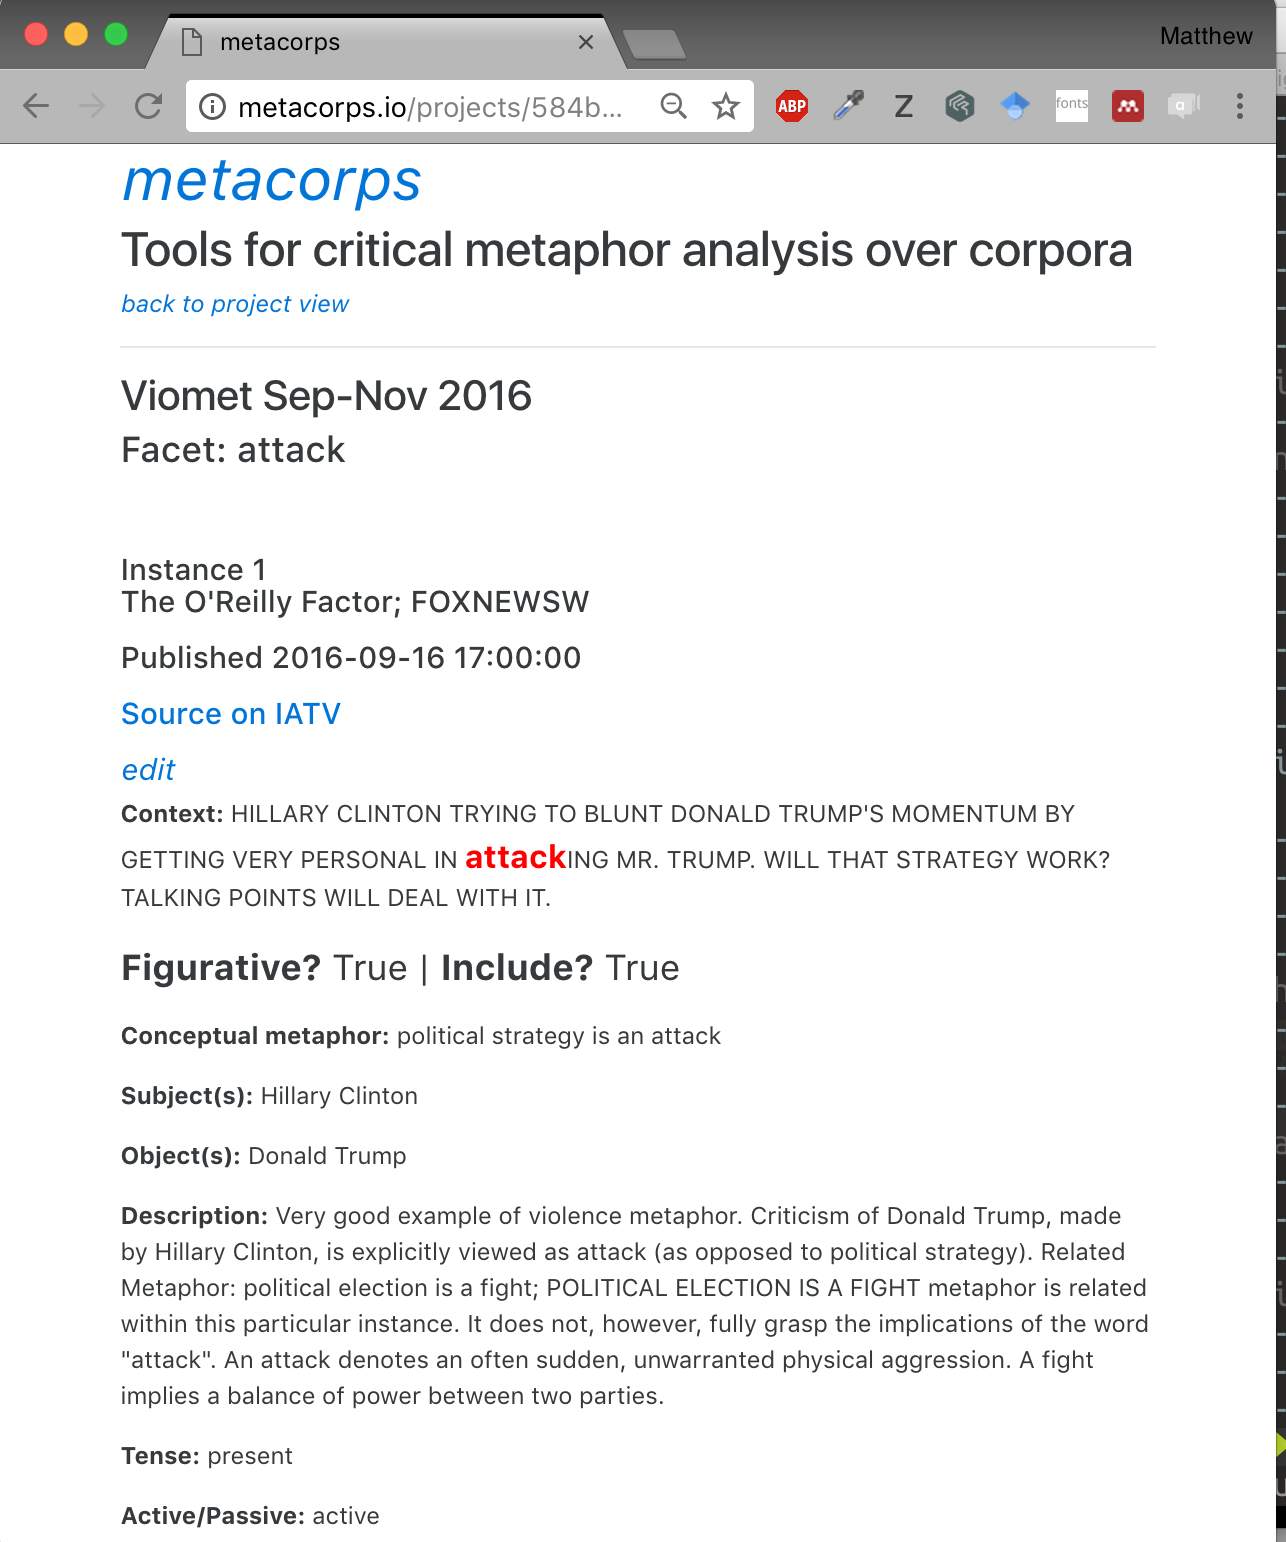
\includegraphics[width=\textwidth]{figures/instances-view.png}}
        \caption{Instance navigation for \textit{attack} facet}
    \end{subfigure}
    ~
    \caption{Screenshots of the Metacorps web app for metaphor annotation over
        corpora}
    \label{fig:metacorps-screenshots}
\end{figure*}

For this project, we had four people contributing to metaphor coding. In order
to keep track of progress and inform others of progress made, the Metacorps
web app includes a user log, shown in Figure \ref{fig:metacorps-home}. 
Once the coders finish annotating a project, it can be exported using an API
that's built-in to Metacorps itself. The user can export the annotations stored
in the database as CSV, or directly to a Pandas \texttt{DataFrame} object
\cite{McKinney2013} for interactive analysis or scripting.

\begin{figure}
    \centering
    \frame{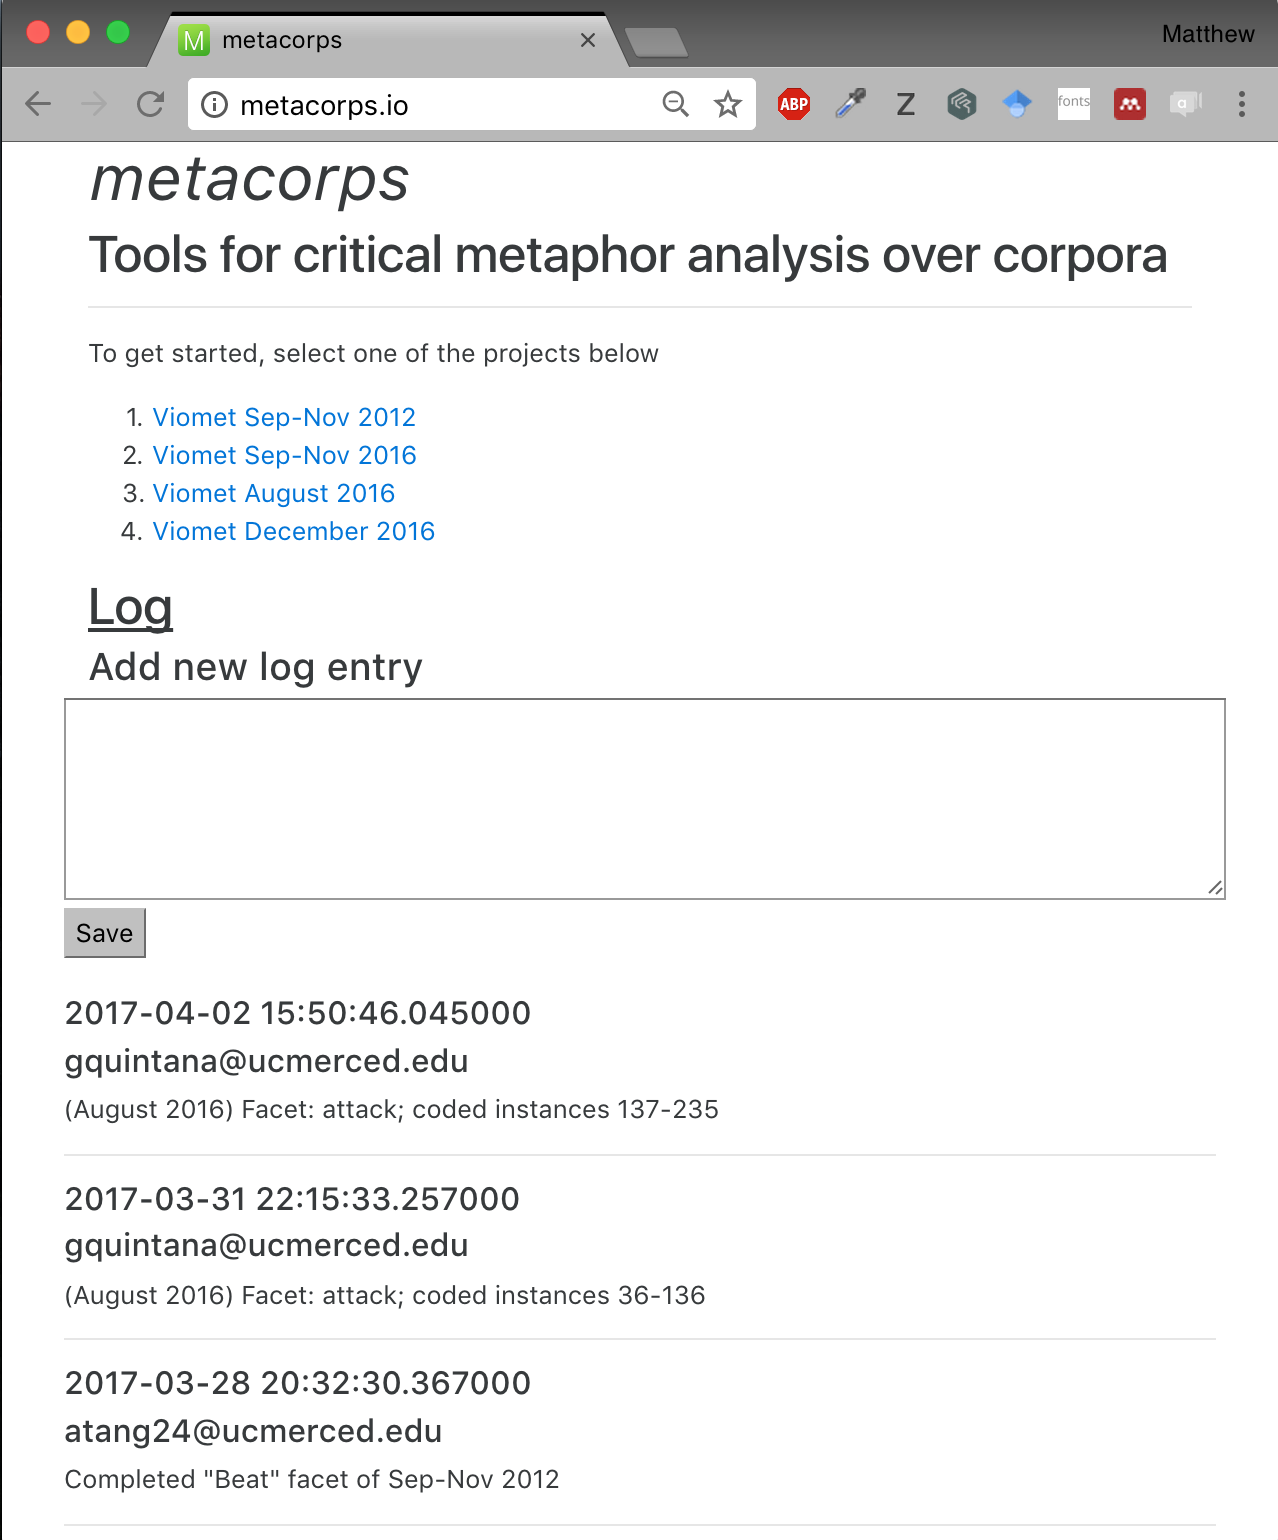
\includegraphics[width=0.75\textwidth]{figures/home-log.png}}
\caption{Home page of Metacorps web app. The metaphor coders use the log to
    inform others of progress. This is just the first step in making the
    app more social and collaborative.}
\label{fig:metacorps-home}
\end{figure}


\subsection{Statistical Analysis}
\label{sub:statistical-analysis}

To review, the goal of the statistical analysis is to determine if and when
phase transitions occur to or from higher or lower frequency of use 
of figurative violence
during the campaign. Preliminary analyses of the data revealed that by far
the most commonly used violent words in figurative violence constructions were
\textit{attack}, \textit{hit}, and \textit{beat}. In order to have higher 
counts and increase statistical power, usages were summed across all programs,
so each day we counted the total number of uses of each one of those words.
There is a sampling of this data table in Table \ref{tab:sample-data}. In 
order to assign phases one, two, and three to each row of this table, we
must first decide what candidate dates we should use for the first and
second phase transition. Part of the analysis is to find what the optimal 
dates are in terms of relative likelihood that the model with two particular
phase transition dates captures more information than any other candidate
model, including the null hypothesis, or no dependence on phase.

\begin{table}[ht]
    \centering
    \begin{tabular}{|r|cc|}
        \hline
        date       &   facet    &  count     \\
        \hline
        2016-09-01 &     attack &    0     \\
        2016-09-02 &     hit    &    1     \\
        2016-09-03 &     hit    &    2     \\
        2016-09-04 &     beat   &    0     \\
        2016-09-05 &     beat   &    1     \\
        $\vdots$   &  $\vdots$  & $\vdots$ \\
    \end{tabular}
    \caption{Example first five rows of data used in statistical analysis to find
    phase transition before addition of phase}
    \label{tab:sample-data}
\end{table}

\begin{table}[ht]
    \centering
    \begin{tabular}{|r|ccc|}
        \hline
        date       &  phase  &   facet    &  count     \\
        \hline               
        2016-09-01 &    1    &     attack &    0     \\
        2016-09-02 &    1    &     hit    &    1     \\
        2016-09-03 &    1    &     hit    &    2     \\
        2016-09-04 &    1    &     beat   &    0     \\
        2016-09-05 &    1    &     beat   &    1     \\
        $\vdots$   & $\vdots$&  $\vdots$  & $\vdots$ \\
    \end{tabular}
    \caption{Example first five rows of data used in statistical analysis to find
    phase transition with addition of phase}
    \label{tab:sample-data-wphase}
\end{table}


To model the data we used general linear mixed models, 
with \texttt{phase} and \texttt{facet} 
being fixed effects. Because the data is count data, Poisson regression was
used. Because there could be fluctuations on any given day,
\texttt{date} is modeled as a random effect. Including random effects are
preferred to simply averaging as this results in less information loss
\cite{Winter2013, Burnham2011, Clark1973}. Model generation was done with
the \texttt{lme4} R package \cite{Bates2015} called seamlessly 
from Python using the \texttt{rpy2} package \cite{Gautier2017}. To summarize,
the two basic models tested are given in Table \ref{tab:models}. The 
theoretical and methodological innovation presented here is in building 
a series of 266 models with 14 candidate dates for the first phase transition
and 19 candidate dates for the second phase transition\footnote{More were
tested in preliminary stages; these correspond to a more specific region of
interest}. In this way, we are actually comparing 267 models: one is the null
hypothesis, that there is no improvement in model performance if we do not
include phase in the model. The 266 other models include phase in the model,
but the dates where we assign each phase are shifted. We performed preliminary
analysis to determine that it was significant to add \texttt{facet} as a 
fixed effect.

\begin{table}[ht]
    \centering
    \begin{tabular}{|r|c|}
        \hline
        description & formula \\
        \hline
        null model, facet only & \texttt{count $\sim$ facet + (1|date)} \\
        includes phase       & \texttt{count $\sim$ phase + facet + (1|date)} \\
        \hline
    \end{tabular}
    \caption{Two basic models considered for modeling figurative violence usage}
    \label{tab:models}
\end{table}

While one could use the chi-square test and significance values to evaluate
the improvement from one model to another, this becomes unwieldy and 
questionable when comparing 267 models. A more modern approach is to compare
the Akaike information criterion (AIC) of the models 
\cite{Akaike1974, Burnham2004, Burnham2011}. The AIC is a measure of 
information loss in a model. It has no meaning on its own, but it is instead
used to calculate the likelihood that another candidate model minimizes 
information loss better than the model with minimum AIC, or 
AIC$_{\mathrm{min}}$. Comparing model $i$ with AIC larger than 
the model with AIC$_{\mathrm{min}}$ is done by calculating the 
the relative likelihood, given by

\begin{equation}
    \mathcal{L}_i = \exp{\left(
      \frac{\mathrm{AIC}_{\mathrm{min}} - \mathrm{AIC}_{i}}{2} 
      \right)
      }
  \label{eq:relative-likelihood}
\end{equation}

\noindent
so called because it yields the probability that model $i$ is actually the one
that results in a lower information loss than the model with AIC$_{\mathrm{min}}$.


In Section \ref{sec:Results}, Figures \ref{fig:AICs} and \ref{fig:relative-likelihoods}
show graphically the calculations of the AIC for all candidate phase
models and the relative likelihood of each candidate phase model, respectively.


\section{Results}
\label{sec:Results}
With the statistical and analytic machinery in place, the results are 
rather straight-forward. However, the results are also rather striking. 
First, as discussed in Section \ref{sec:Methods}, we computed the mixed model
given by \texttt{count $\sim$ phase + facet + (1|date)} for 266 different date
partitions determining which date was assigned to which phase. The first
partition date ranged between September 26 and October 9, 2016. The
second partition date was between October 27 and November 14, 2016.
The phase was 1 if the date was before the first partition date, 2 if the 
date was on or after the first partition date and before the 
second partition date, or 3 if the observation date was on or after the second 
partition date.


\begin{figure}
  \centering
  % \vspace*{-.55in}
  \hspace*{-.25in}
  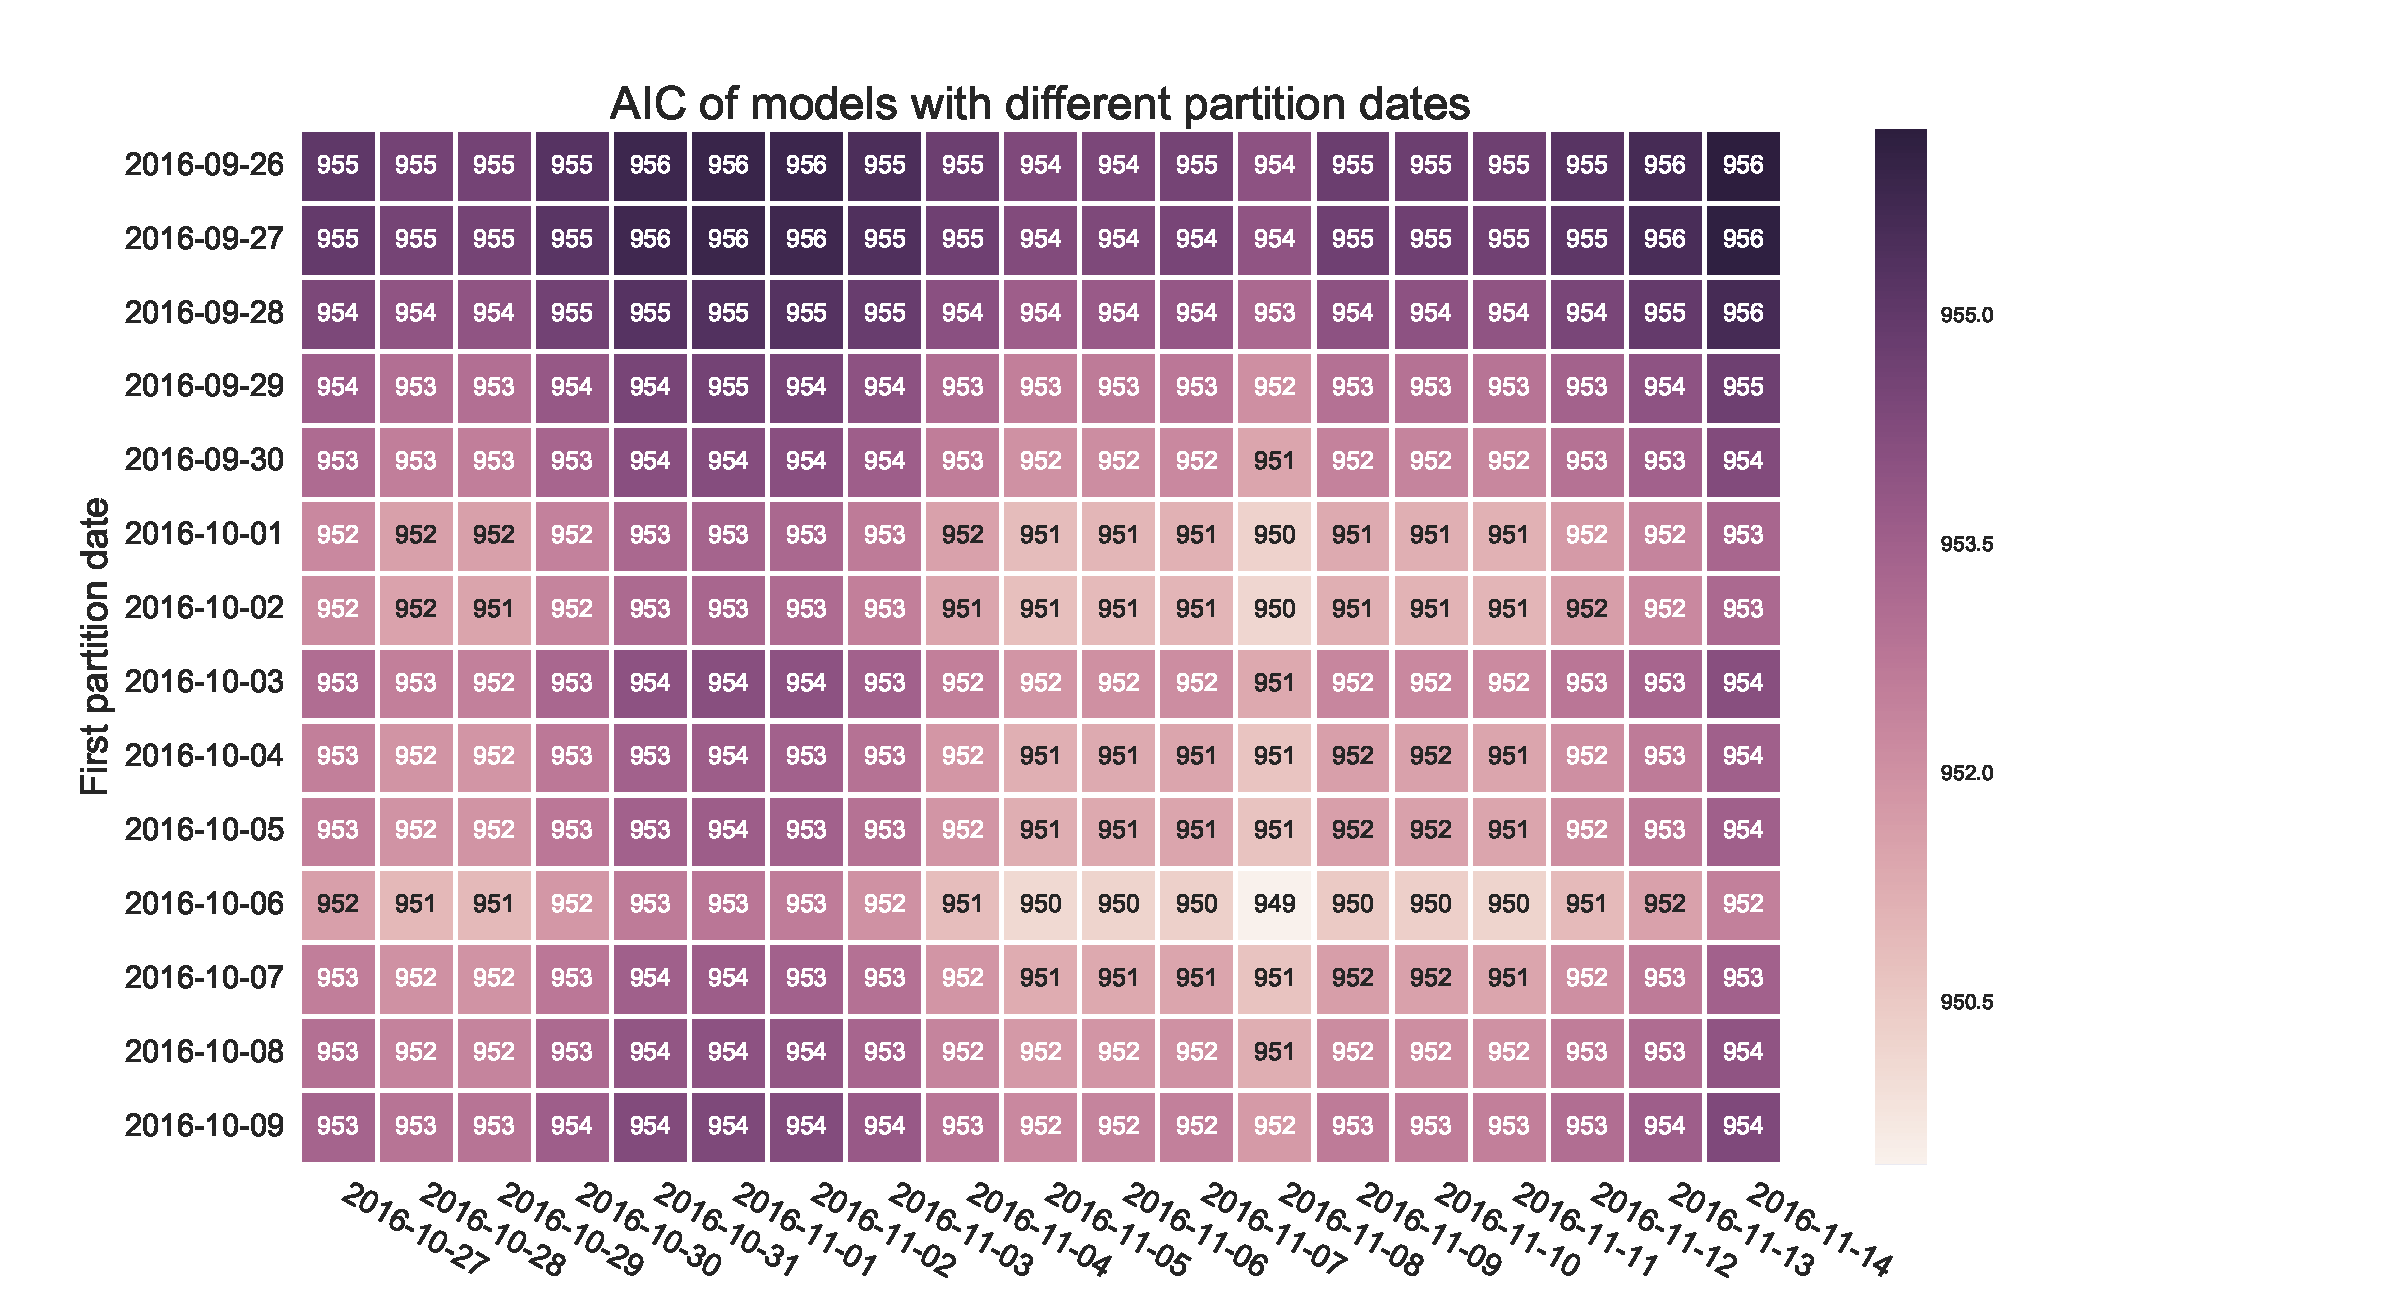
\includegraphics[width=1.25\textwidth]{figures/AIC_dates-FIG2.pdf}

\caption{
  Akaike information criterion (AIC) for models of \texttt{count $\sim$ phase + facet + (1|date)}
  for 266 different phase assignments. The phase was 1 if the date was before
  the first partition date, 2 if the date was on or after
  the first partition date and before the second partition date, or
  3 if the observation date was on or after the second partition date.
}
\label{fig:AICs}
\end{figure}


\begin{figure}
  \centering
  % \vspace*{-.55in}
  \hspace*{-.25in}
  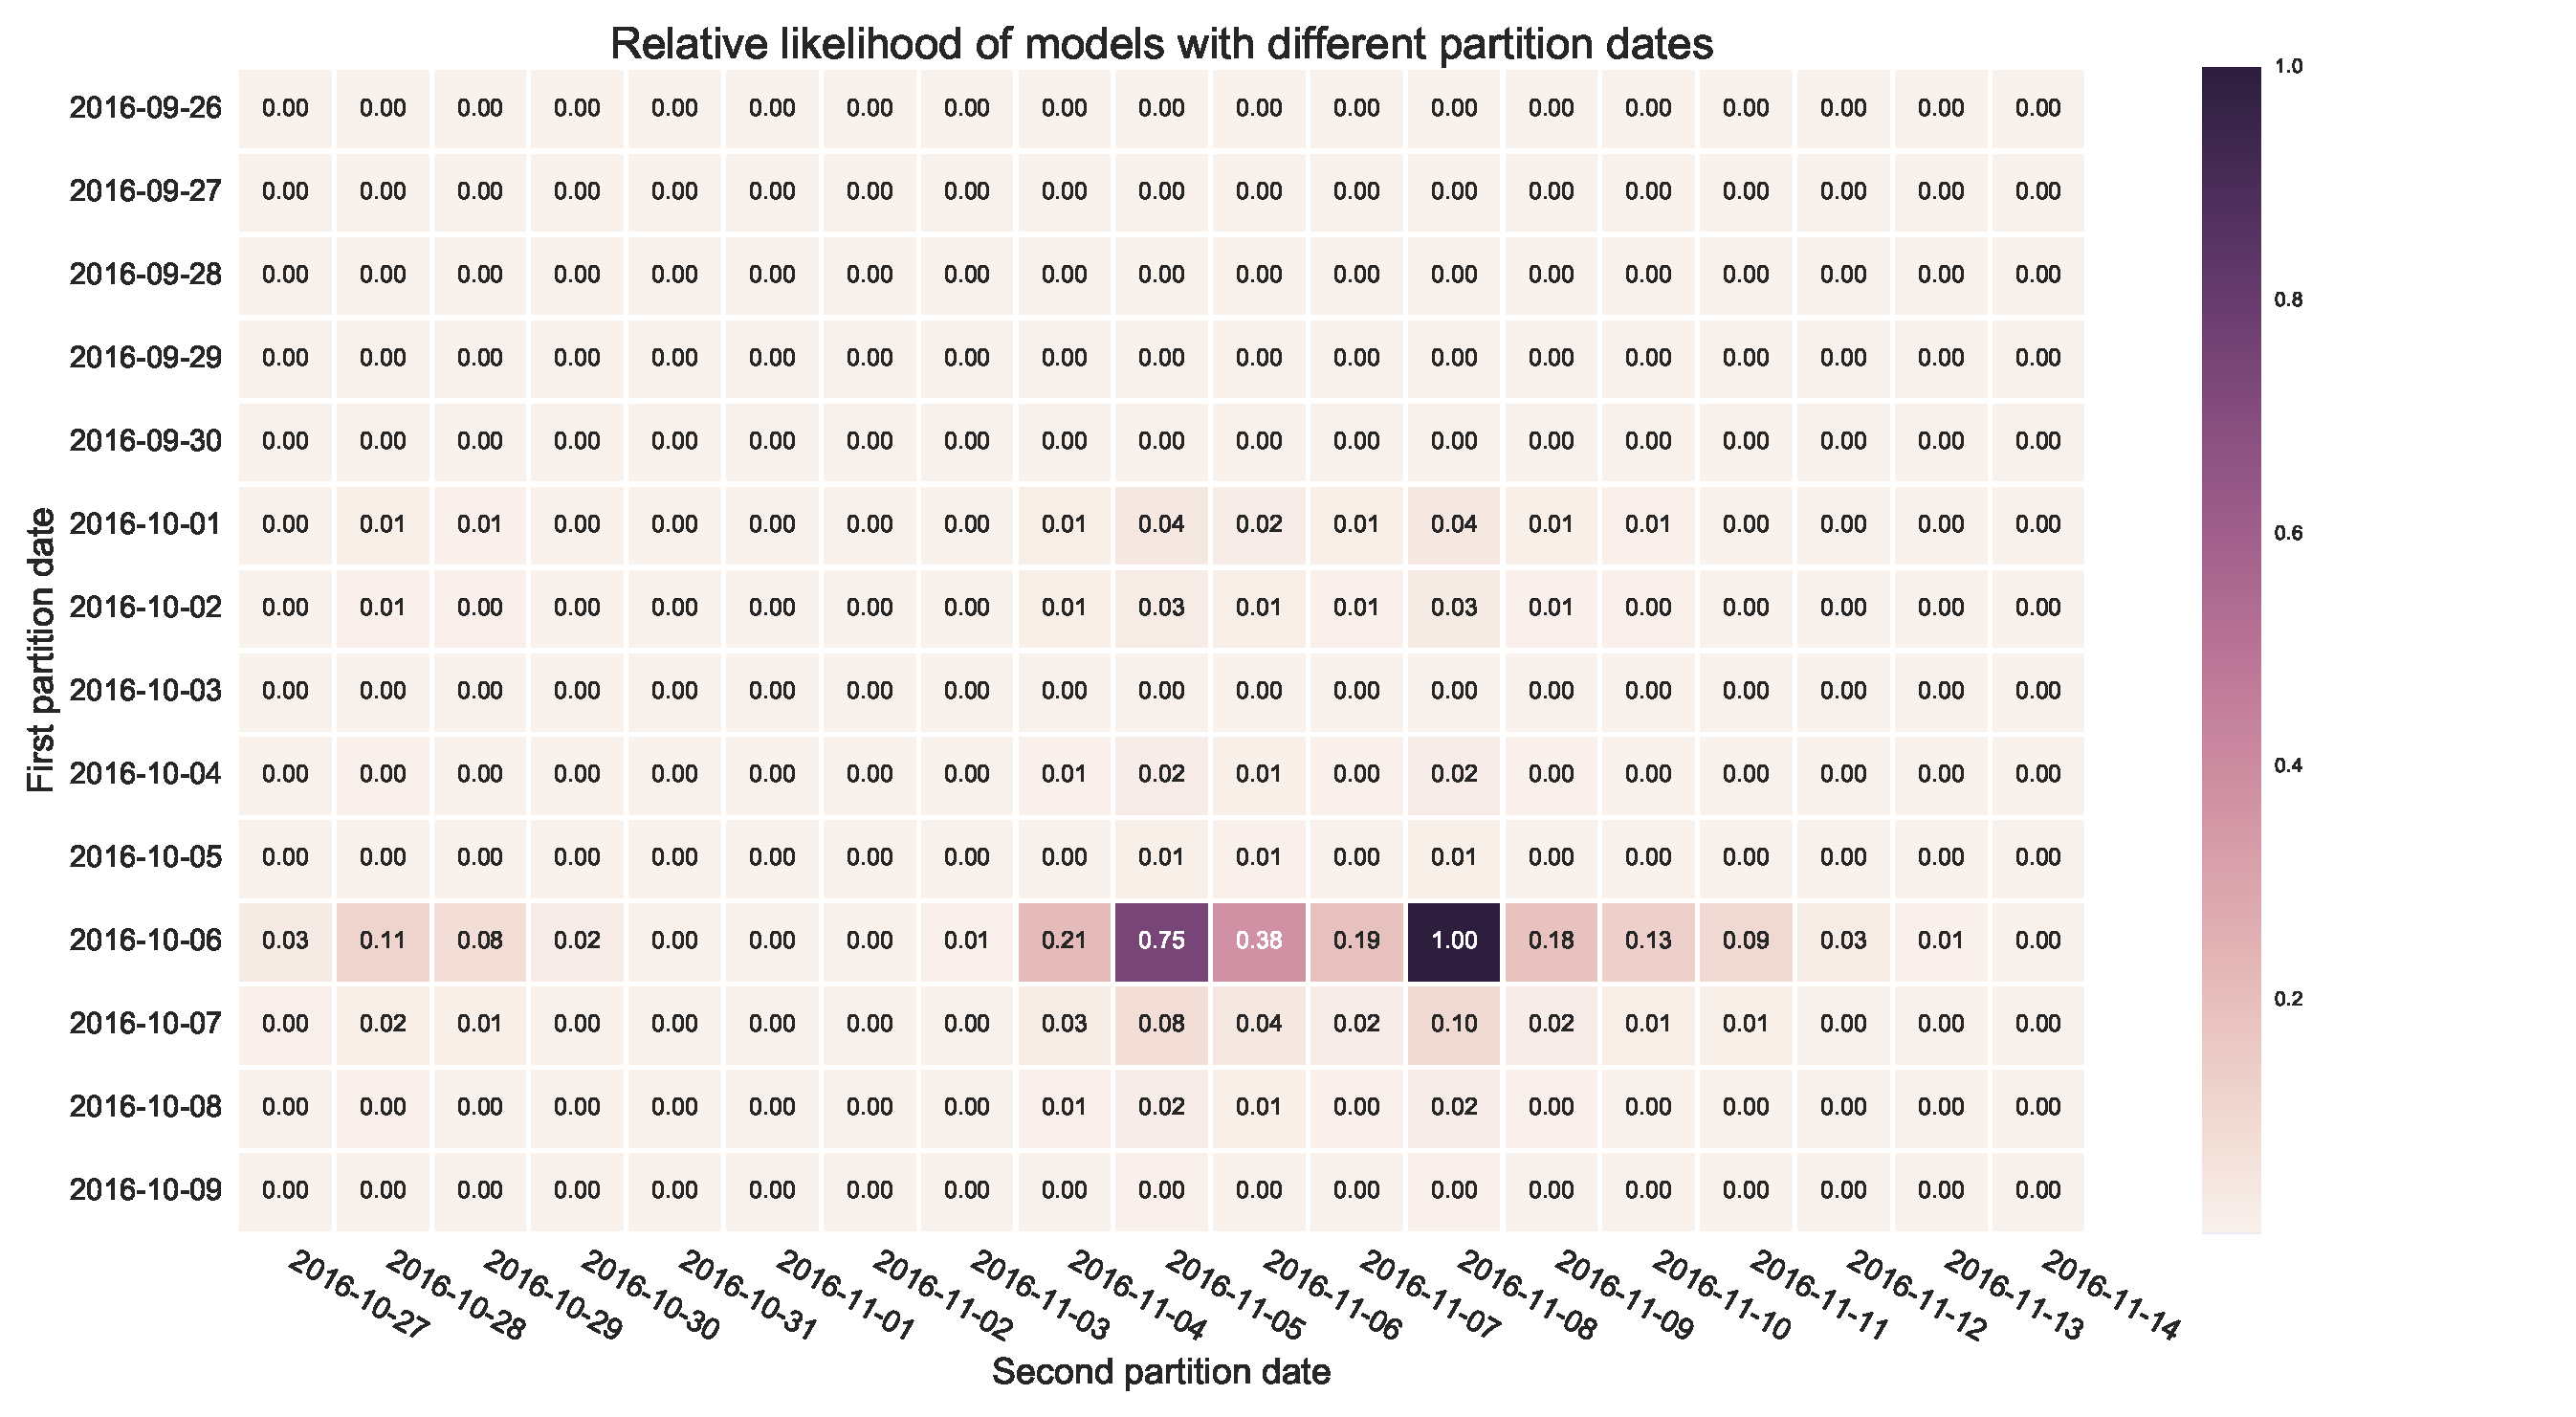
\includegraphics[width=1.25\textwidth]{figures/rel_likelihood_dates-FIG2.pdf}

\caption{
  Relative likelihood of models with identical formula, but different dates
  used to partition the data into three ``phases''. The phase 
  was 1 if the date was before
  the first partition date, 2 if the date was on or after
  the first partition date and before the second partition date, or
  3 if the observation date was on or after the second partition date.
}
\label{fig:relative-likelihoods}
\end{figure}

Recall that a model with relatively higher AIC means more information was lost by
that model. So, a lower relative AIC is better. However, miniscule differences
in AIC cannot be considered conclusive. To select the model that best fits the
data, which in turn selects the dates that best correspond to the locations
of the phase transitions, we first compute the AIC of all candidate models, 
The results of this calculation for all candidate models that include phase
are shown in Figure \ref{fig:AICs}. To determine the probability that 
another model will not minimize information loss better,
the model with the minimum AIC is compared to all $N-1$ other models using
the relative likelihood, $\mathcal{L}_i$, where $i = 1, \ldots, N;~i \neq i_{min}$,
where $i_{min}$ is the model index with minimum AIC. $\mathcal{L}_i$ was defined
in Equation \ref{eq:relative-likelihood}. 

The pair of partition dates with the smallest AIC was October 10 and
November 8, with an AIC of 949. We then calculated $\mathcal{L}_i$ for all 
$N-1$ other models, 
with the results shown in Figure \ref{fig:relative-likelihoods}. At first,
we might be discouraged by the results. While the we do find a minimum
AIC that is significantly less than the null model 
($\mathrm{AIC}_{\mathrm{null}} = 955.63;~\mathcal{L}_{\mathrm{null}} = .046$),
there are many candidates with high relative likelihoods. 
There is a explanation that does not imply that our method for
identifying the location of a phase transition is not working. What if,
instead, our procedure is identifying an area of mixed phase, or a transient
phase to use more of a dynamical systems term. 


\section{Discussion}
We have shown that average figurative violence usage increases after the
debates begin. We have also shown that this increase in usage decreases
significantly by the election, November 8, 2016. The onset of the increase
seems, then, to lag the first debate by about eleven days. Although our analysis
did identify a single best labelling for each phase, there were other candidates
that were nearly as likely to be the optimal fit to the data. We can think of
this as either the chosen partition dates to not be too significant in 
modeling changes in figurative violence usage. Or, we could push our 
dynamical systems approach further and think about these in terms of transience.
Just like circuits show a particular rise time and settling time in response
to the application or reduction of electric potential, we might interpret this
uncertainty in partition dates as the system of cable news production to be
indicative of a ``rise'' to its equilibrium state in response to the rise in
the ``impulse'' of the onset of presidential debates.

This result is not just of theoretical importance. Anthropologist
Arlie Russel Hochschild recently published a book \textit{Strangers in their
Own Land} which carefully studied the increasing animosity and 
polarization of American politics and political discourse \cite{Hochschild2016}.
To describe the problem we are all facing, Hochschild 
describes the political left and right as being on opposite sides of
an ``empathy wall'', a poignant metaphor. 
This wall is made ever higher by geographic clustering of likeminded people,
personalized media tailored to fit and deepen pre-existing political biases, and other 
factors. It seems the physiological and neurological impact of metaphorical
violence would only increase the height of this empathy wall between fellow citizens at a time
when we desperately need the wall lowered.

Believing that the political left is superior, cognitive linguist George Lakoff
argues in a series of books that the path to a better United States is 
one where progressives give voice to their values 
\cite{Lakoff1996, Lakoff2004, Lakoff2008, Lakoff2012}. 
This may or may not be true, 
but these works are accompanied by broad-brush, nonrigorous claims about United
States citizens' conceptual wordviews. For example, a central
claim to the series of political writings cited above 
is that ``conservative and progressive politics are organized around 
two very different models of married life: a strict father family and a 
nurturant parent family'' \cite[p.47]{Lakoff2004} But
under what circumstances does this claim hold, if the claim is even detailed
enough to hold in any meaningful sense at all? The results we demonstrate
support a claim advocated since at least \citeA{Gibbs1997} 
encouraged us to take ``metaphor out of our heads and into the cultural
world'' that 
we cannot separate our metaphors from their environment. So even if in some
broad sense Lakoff's claim is true, there are subtleties of ``progressives''
and ``conservative'' conceptual worldviews that must be in constant flux.

Instead, I am inspired by Hochschild's desire to understand the structure
of the empathy wall and to find ways to get over it or to lower it. By better
understanding what cultural events give rise to harmful talk that further vaults
the empathy wall, we can suggest better alternatives. This approach brings
more rigor to the study of pragmatics in political talk, and reveals the
deep connection between certain cultural events and our use of metaphorical
violence. It is a promising method for identifying other metaphorical 
constructions in relation to other cultural events.

Future work should first include longer timescales and other situations. For
example, we should see if there are other detectable transitions when the national 
conventions and the preliminary debates were happening. These results 
should be compared to the same three months for the 2012 elections. There is
also much more to be done with the other data collected in the analysis of 
these three months. How does the source domain change over time? That is, 
what is the nature of the metaphorical violence? For example, does
the ratio of uses of \textit{attack} to \textit{hit} change
with each phase, for example? Would such a ratio show phase transitions
at different times? Or are some ratios fixed, with no significant phase
transition? How does tense change over time? Who is most often the subject
or object of metaphorical violence? Do subject/object relationships also
show phase transitions? Answering these and similar questions may enable us
to better prepare for and understand pragmatic ``choice'' in political talk, 
and advocate for and make pragmatic decisions that can result in less division
and more empathy in politics in general.



\bibliographystyle{apacite}

\setlength{\bibleftmargin}{.125in}
\setlength{\bibindent}{-\bibleftmargin}

\bibliography{/Users/mt/workspace/papers/library.bib}

% \appendix

% \section{Software}
% In the course of this project I developed open-source software tools and
analysis scripts. The \texttt{iatv} package provides an API to programmatically
scrape the Internet Archive's TV News Archive (TVNA). \texttt{Metacorps}
provides methods for searching for potential metaphor, loading all potential
metaphor into a database, collaborative coding the potential metaphor in a 
browser-based app, and a data analysis pipeline for the coded metaphors. 

\subsection{iatv: open source tool for TVNA scraping}
\label{subsec:iatv}

To access the data on the TVNA, I developed a new, open-source 
software tool in the Python programming language called \textit{iatv}
\cite{Turner2016}. More details can be found on the GitHub repository page
at \url{http://github.com/mtpain/iatv}. But as a brief example, here is
how one would download all transcripts and the associated metadata from
all shows aired on Fox News in September, 2016

\begin{minted}[fontsize=\small]{python}
from iatv import search_items, download_all_transcripts

# search string cannot be empty so use 'I'; set rows=1000 to get all shows 
items = search_items('I', channel='FOXNEWSW', time='201609', rows=1000)

# filter out commercials
shows = [item for item in items if 'commercial' not in item]

# base_directory will be created or overwritten by default
download_all_transcripts(shows, base_directory='FOXNEWSW-Sep2016')
\end{minted}

Here is an example of the directory structure of \texttt{base\_directory}, which
has been set to \texttt{FOXNEWSW-Sep2016}.

{\small
\begin{verbatim} 
FOXNEWSW-Sep2016
|
+-FOXNEWSW_20160901_000000_The_OReilly_Factor
|   |
|   +-FOXNEWSW_20160901_000000_The_OReilly_Factor.cc5.srt
|   +-metadata.json
|   +-transcript.txt
|
+-FOXNEWSW_20160901_010000_The_Kelly_File
|   |
|   +-FOXNEWSW_20160901_010000_The_Kelly_File.cc5.srt
...
\end{verbatim}
}

\noindent
The \texttt{base\_directory} is populated with subdirectories named by the Internet
Archive's ID for the program. Within each of those subdirectories, there is
the raw \texttt{.srt} file, containing the SubRip-formatted captions 
\cite{Matroska2016}, a metadata file containing all metadata obtained from the
TVNA, and a text file of the transcript converted from the \texttt{.srt} using
\href{https://github.com/pbs/pycaption}{PBS's \texttt{pycaption} library} for Python
\cite{PBS2016}. This concludes the first step in the data acquisition and
processing pipeline, continued in the following sections.


\subsection{Metacorps: Web app and API for corpus annotation and analysis}
\label{sub:corpus-annotation}

Here we introduce the web application and underlying data model that allows us
to collaboratively code instances of metaphor using the \texttt{FOXNEWSW-Sep2016} as
an example. This process is implemented using the 
\href{http://github.com/mtpain/metacorps}{\texttt{metacorps} package} I developed
as part of this project \cite{Turner2017}. 
The package includes both the web application
front-end for collaborative metaphor coding and an API for building the 
specific datasets to be analyzed, including searching for relevant violent
words and phrases. 

In the first step of this process, we insert the data and metadata
acquired from the TVNA into a MongoDB database. No further pre-processing is done 
at this point.
Each subdirectory in the \texttt{FOXNEWSW-Sep2016} is considered an \texttt{IatvDocument},
which is represented as a Python class. All MongoDB collections are represented
as Python classes, using the \texttt{mongoengine} document-object mapping software
\cite{Mongoengine2017}. Then specific documents are selected for analysis, 
building a separate corpus under the collection \texttt{IatvCorpus}. 
An \texttt{IatvCorpus} is then used to build another collection type, a
\texttt{Project}. In building the project, a list of 
violent words or phrases that may be used figuratively must also be given.
Each of these words defines a \texttt{Facet}, and each \texttt{Facet} is comprised
of a list of \texttt{Instance} types. Instances are potential figurative uses
of violence. These instances are what are reviewed by annotaters.
In the web interface, the reviewers can read the paragraph in which the
instance occurred, mark whether the instance was indeed figurative, whether to
include it in the analysis (it may be figurative but not related to politics),
the underlying conceptual metaphor, the perpetrator and victim of violence,
the tense, and whether or not the construction is active or passive. A 
screenshot of the facet navigation page and the \textit{attack} instance
navigation and viewing page are shown in Figure \ref{fig:metacorps-screenshots}.

\begin{figure*}[t!]
    \centering
    \begin{subfigure}[b]{0.45\textwidth}
        \frame{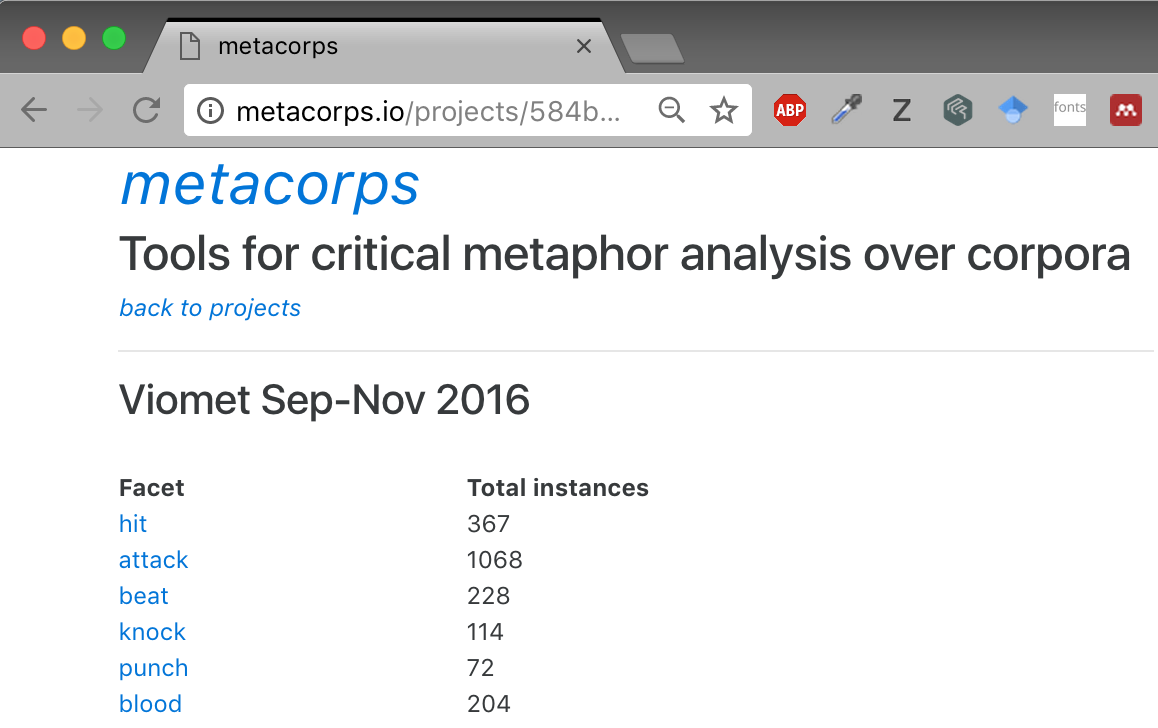
\includegraphics[width=\textwidth]{figures/facet-view.png}}
        \caption{Facet navigation}
    \end{subfigure}
    ~
    \begin{subfigure}[b]{0.45\textwidth}
            \frame{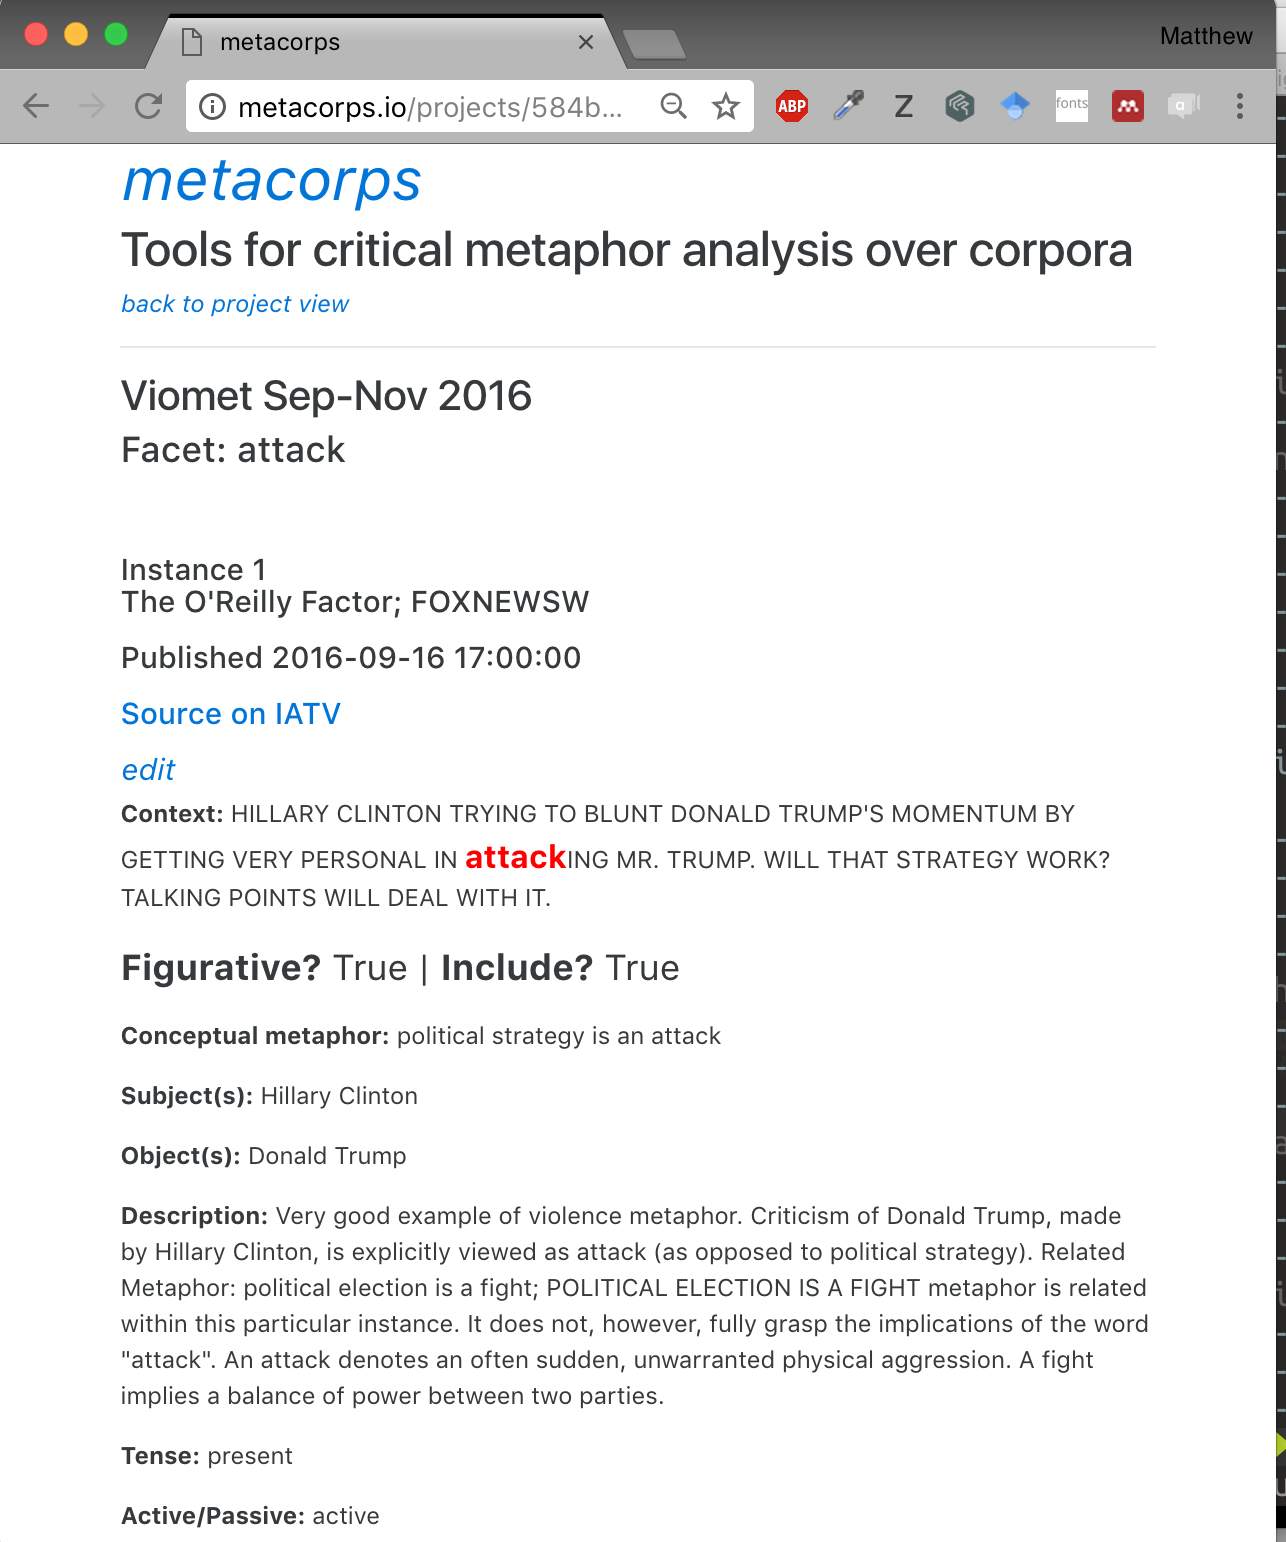
\includegraphics[width=\textwidth]{figures/instances-view.png}}
        \caption{Instance navigation for \textit{attack} facet}
    \end{subfigure}
    ~
    \caption{Screenshots of the Metacorps web app for metaphor annotation over
        corpora}
    \label{fig:metacorps-screenshots}
\end{figure*}

For this project, we had four people contributing to metaphor coding. In order
to keep track of progress and inform others of progress made, the Metacorps
web app includes a user log, shown in Figure \ref{fig:metacorps-home}. 
Once the coders finish annotating a project, it can be exported using an API
that's built-in to Metacorps itself. The user can export the annotations stored
in the database as CSV, or directly to a Pandas \texttt{DataFrame} object
\cite{McKinney2013} for interactive analysis or scripting.

\begin{figure}
    \centering
    \frame{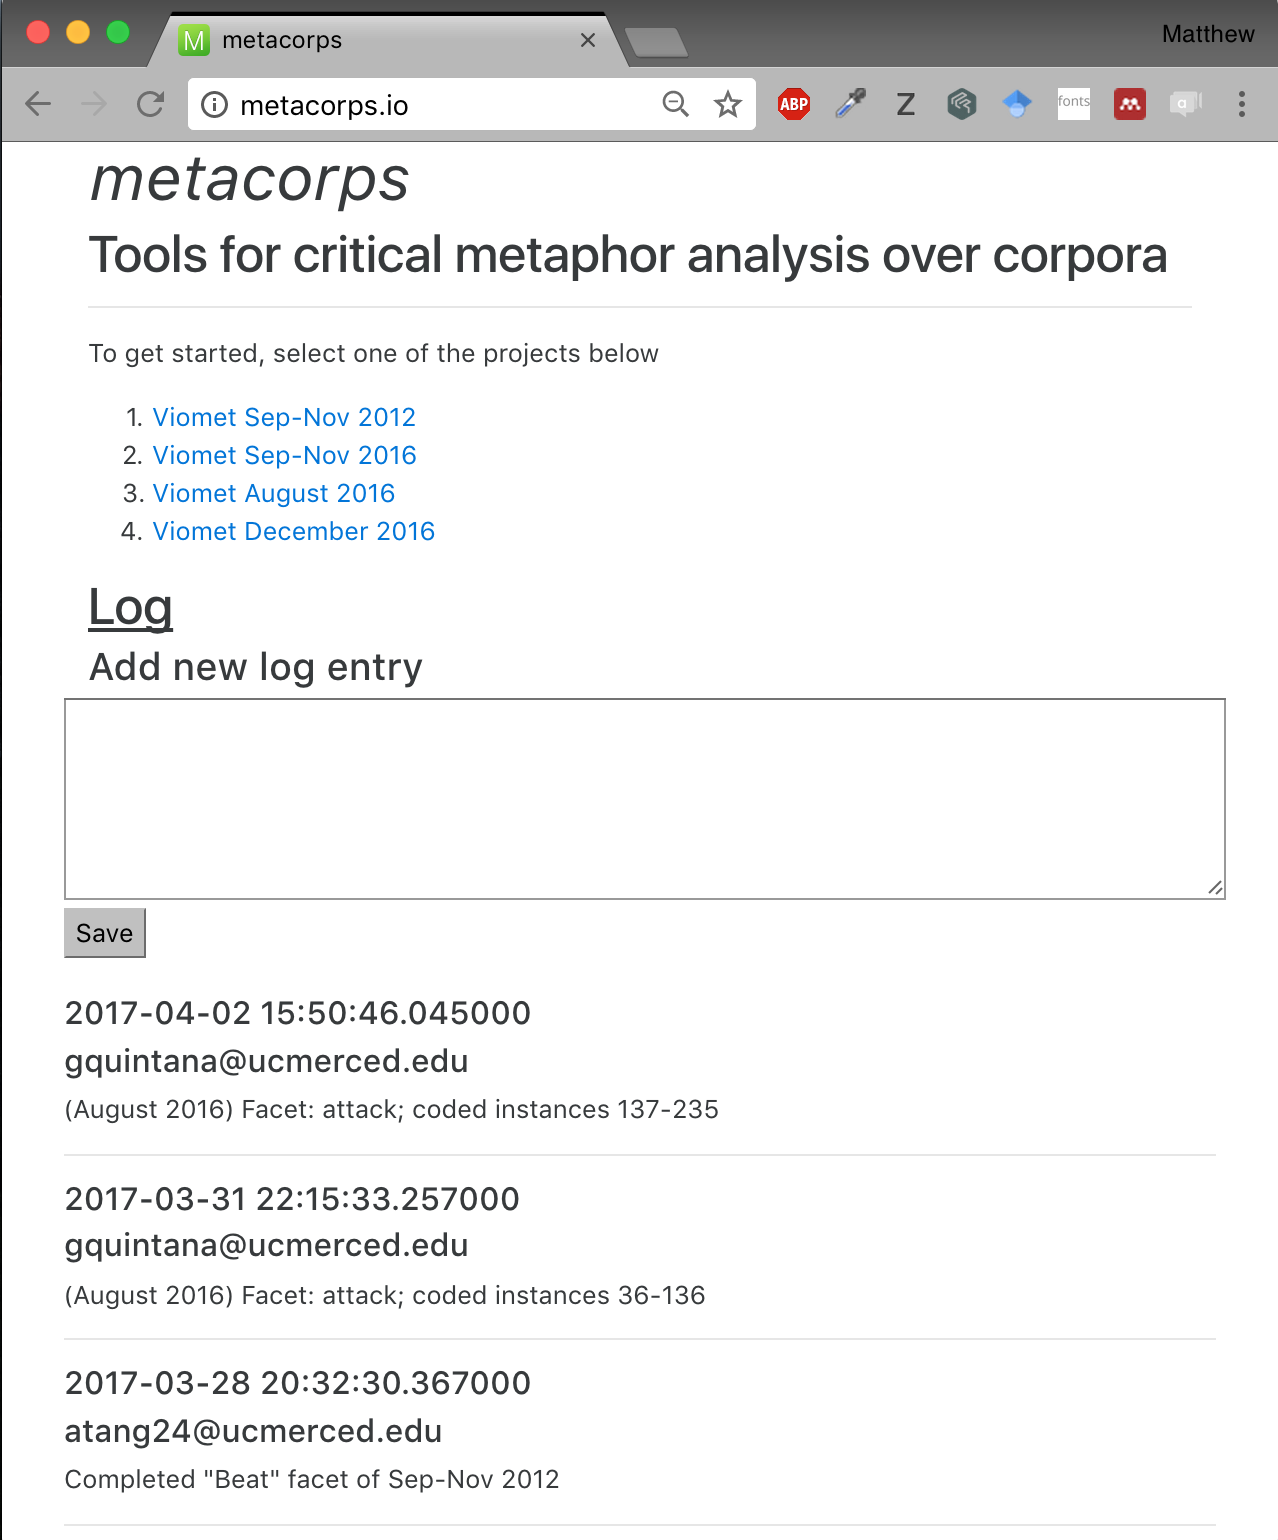
\includegraphics[width=0.75\textwidth]{figures/home-log.png}}
\caption{Home page of Metacorps web app. The metaphor coders use the log to
    inform others of progress. This is just the first step in making the
    app more social and collaborative.}
\label{fig:metacorps-home}
\end{figure}




\end{document}
